\documentclass[10pt,conference,compsocconf]{IEEEtran}

\usepackage{hyperref}
\usepackage{graphicx}
\usepackage{xcolor}
\usepackage{blindtext, amsmath, comment, subfig}
\usepackage{grffile}
\usepackage{caption}
%\usepackage{subcaption}
%\usepackage{algorithmic}
\usepackage[utf8]{inputenc}


\title{CS-523 SecretStroll Report}
\author{Author 1, Author 2}
\date{April 2020}

\begin{document}

\maketitle

\begin{abstract}
    SecretStroll is a privacy preserving LBS. SecretStroll is build on top of 3 core modules: an Anonymous
    \textit{Attribute-based Credential protocol} for authorization, <part 2> and <part 3>.
\end{abstract}

\section{Introduction}
SecretStroll is a Location Based System (LBS), which aims to provide users with information about Points of Interest (POI)
near their location, satisfying user-specified criteria (i.e retrieve POIs near user location which correspond to the description
of "restaurant").\newline
LBS are prone to be privacy-sensitive system: if not implemented following a \textit{Privacy by Design} paradigm, they can leak
many information about users, such as their location and movement patterns, which can lead to more privacy-disruptive disclosure attacks.
For this reason, we designed SecretStroll by identifying layers at which the system could potentially leak information and implementing
privacy-preserving mechanism at each layer.\newline
SecretStroll is formed by 3 core layers: an \textit{Attribute-based Credential} protocol, <part2> and <part3>.
\subsection{Attribute-based credential}
SecretStroll exploits an Attribute-based credential Protocol to authorize users to fetch POIs of a given type, for which they must have subscribed to.
At issuing time, users will provide their username together to a set subscriptions (i.e types of POIs) which are currently supported
by SecretStroll system. SecretStroll server will verify the validity of user's request and generate a valid credential for the specified
subscriptions and username. Users will later show their credentials together with a subset of their subscriptions: in this step,
the \textit{Showing protocol}, users will have to prove to the server to have a valid credential over their attributes
(including, but not limited to, their subscriptions). Users will also use their credential to perform a digital signature
on their current location. If the proof suceeds, the server will reply with a list of POIs matching the types requested by the user.
\subsection{part 2}
\subsection{part 3}
\section{Attribute-based credential}
For the implementation of the authorization through \textit{Attribute-based credentials}, we have carefully followed the protocol
described by \textit{Pointcheval and Sanders} \cite{PS_signature}.
Nevertheless, during the development of the \textit{ABC} system, some design challenges needed to be solve, and it is worth highlighting their solution:
\begin{itemize}
    \item \textbf{Server-Client agreement on the attribute domain}: as described in \cite{PS_signature}, before even starting the protocol,
    server and client must agree on the public parameters, including the number $L$ of possible attributes. Moreover, users should choose
    attributes (subscriptions) which are recognized by the server. To this end, we decided to embed the list of available subscriptions
    in the server public key (which follows the description of the paper). The 'attribute domain' is thus formed by the $L-2$ possible
    subscriptions, followed by the username and, following a common approach in designing \textit{ABC} protocols, a client secret key.
    Clients are expected to choose their subscriptions from the provided set: failing to comply with the protocol on client sidewill result in the
    abortion of the protocol itself by the server.
    \item \textbf{Attribute encoding}: once we designed the server-client agreement in such a way that each parameter of the public key
    (namely $Y_i$ and $\tilde{Y}_{i}$) was mapped to one attribute, we decided to encode attributes in the following way:
    if the user decides to subscribe to service $i$, then the exponent of parameter $i$ of server public key(i.e the attribute),
     will be a fixed prime number in $Z_p$ (where $p$ is the order of the prime groups defined in the paper),
    to which we refer as \texttt{SUBSCRIBED\_YES}. Conversely, any service to which the client does not subscribe,
    will be encoded with a different fixed prime, \texttt{SUBSCRIBED\_NO}. The 'username' attribute will be encoded through
    \texttt{int.from\_bytes(username.encode(), 'big')} method available in \texttt{python}. Client secret key will be a
    random number in $Z_p$.
    \item \textbf{Fiat-Shamir Heuristic for Issuance Request}: the \textit{Issuance Protocol} once again follow thoroughly the paper description.
    Client will choose their \textit{user-defined} attributes, which in our implementation will simply be its secret key,
    togheter with a blinding factor $t$. Note that the random blinding factor guarantees \textit{issuer unlinkability}. User commitment $C$ will thus be $g^{t}*Y_{L}^{client\_sk}$. Client will also produce a
    \textit{Non Interactive Zero Knowledge Proof of Knowledge} of his commitment. In order to generate the challenge in a
    non interactive way, we applied \textit{Fiat-Shamir Heuristic} to the \textit{sigma protocol} defined for the
    \textit{Pedersen's Commitment Proof of Knowledge}: the provided challenge was the \textit{sha256} digest of the public parameters
    (the commitment $C$, the randomness $R$ of the proof, and the public key parameters used for exponentiation, $g$ and $Y_{L}^{client\_sk}$)
    \item \textbf{Fiat-Shamir Heuristic for linking Disclosure Proof to location}: \textit{Fiat Shamir Heuristic} plays also a crucial role when
    linking the \textit{Showing protocol} of the paper to a specific message (i.e client's current location). This prevents a malicious user
    eavesdropping communication to steal one user's credential in order to gain access to the service from its current location.
    In order to apply \textit{Fiat-Shamir Heuristic}, we modelled the \textit{Disclosure Proof} as a regular \textit{NIZKP} on a Pedersen's Commitment,
    where generators belong to the $G_T$ group.\newline
    In this specific setting, the user commitment is: \[C=e(\sigma_{1}^{`}, \tilde{g})^t\prod_{i \in H}e(\tilde{Y}_{i}^{a_i},\tilde{g})\]Thus,
    the generators in the Proof of Knowledge are $e(\sigma_{1}^{`}, \tilde{g})$ and $e(\tilde{Y}_{i}^{a_i},\tilde{g})$.
    In order to link the location to the proof, we used a \textit{Schnorr's Signature}, producing the challenge as:
    \[c = sha256(R|C|public\_parameters|location)\]
    The server validations follows two steps: first, it checks it can recompute client's commitment via the \textit{bilinear} property of the pairing:
    \[C = e(\sigma_2^`,\tilde{g})\prod_{i \in D}e(\sigma_1^`,\tilde{Y}_i)^{-a_i}e(\sigma_1^`,\tilde{X})^{-1}\]
    Secondly, it checks the validity of the proof on client's commitment. Also, it is worth noticing that the \textit{ABC} protocol fulfills both selective disclosure and, thanks to the randomization of the signature $\sigma$, verifier unlinkability.
\end{itemize}
\subsection{Test}
In order to test the correctness of our \textit{ABC protocol}, we implemented a simple test suite using \texttt{pytest} called \texttt{test\_abc.py},
involving a correct run of the protocol and 4 runs where the client deviate from the protocol in different ways:
\begin{itemize}
    \item \texttt{test\_registering\_invalid\_attributes}: client issues a request with an attribute which do not belong to the agreed domain.
    \item \texttt{test\_requesting\_service\_not\_subscribed}: client tries to request a service to which it did not subscribe.
    Implicitly, this will lead to a \textit{Disclosure Proof} which is not valid for the given credentials.
    \item \texttt{test\_invalid\_signature\_on\_message}: simulates a passive adversary who is able to eavesdrop
    communication between another user and the server, trying to ask for a given service, from its current
    location, by replaying the \textit{Disclosure Proof} sent by a client from a different location.
    \item \texttt{test\_invalid\_user\_commitment}: when creating the issue request, client presents a proof which is not valid for his commitment.
\end{itemize}

\subsection{Evaluation}
For the evaluation of the \textit{ABC protocol}, we analyzed how the communication cost in terms of exchanged bytes, and the
computational cost in terms of runtime, variate in respect to the number of available subscriptions (attributes). The analysis has
been repeated seperatelly for each of the steps:
\begin{figure}[h!]
    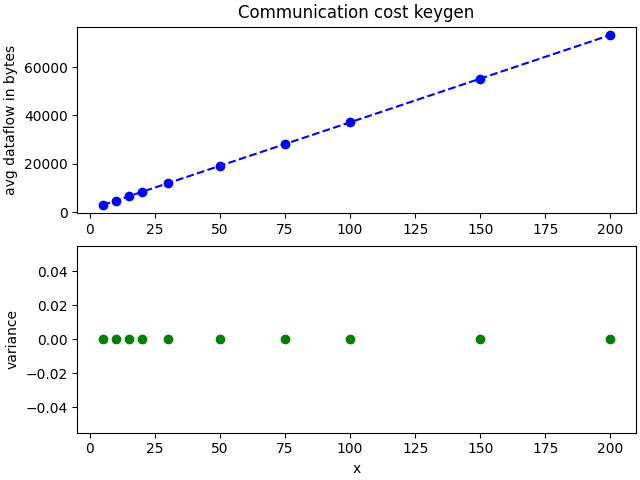
\includegraphics[width=0.49\linewidth]{../performance_analysis/dataflow_keygen.png}
    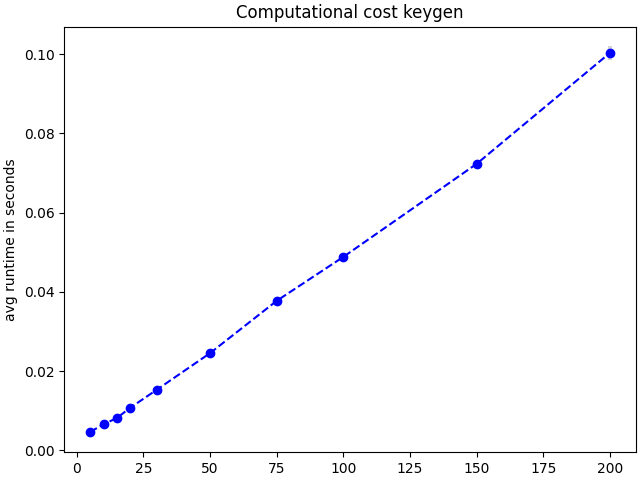
\includegraphics[width=0.49\linewidth]{../performance_analysis/runtime_keygen.png}
    \caption{Avg dataflow and runtime for the key generation step}
    \label{fig:keygen}
\end{figure}

\begin{figure}[h!]
    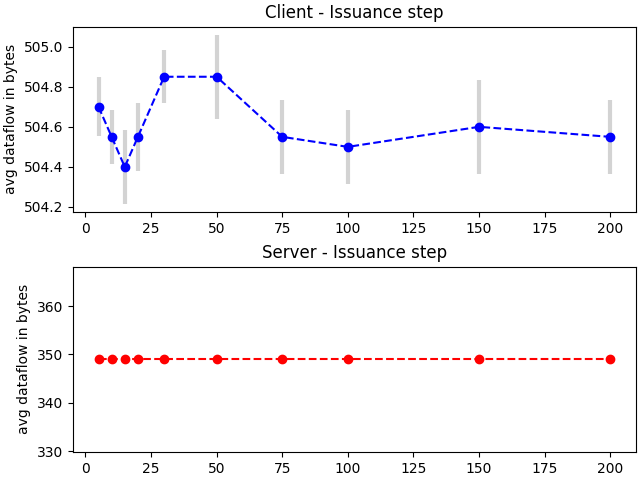
\includegraphics[width=0.49\linewidth]{../performance_analysis/dataflow_issuance.png}
    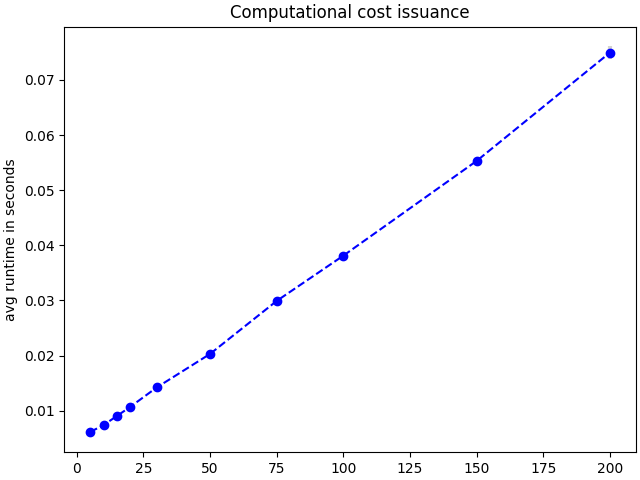
\includegraphics[width=0.49\linewidth]{../performance_analysis/runtime_issuance.png}
    \caption{Avg dataflow and runtime for the credential issuing process}
    \label{fig:issuance}
\end{figure}


\begin{figure}[h!]
    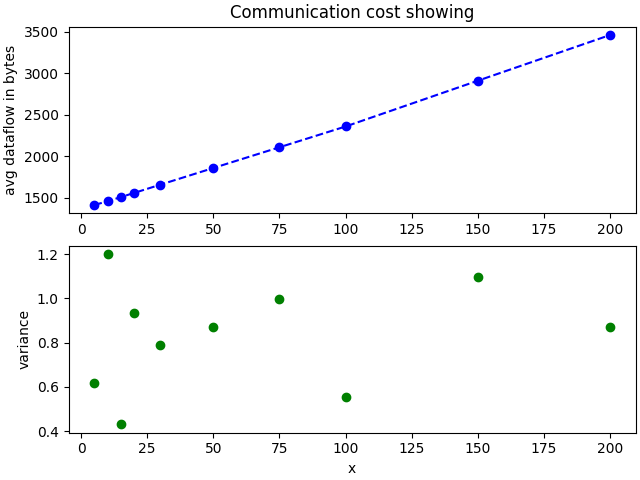
\includegraphics[width=0.49\linewidth]{../performance_analysis/dataflow_showing.png}
    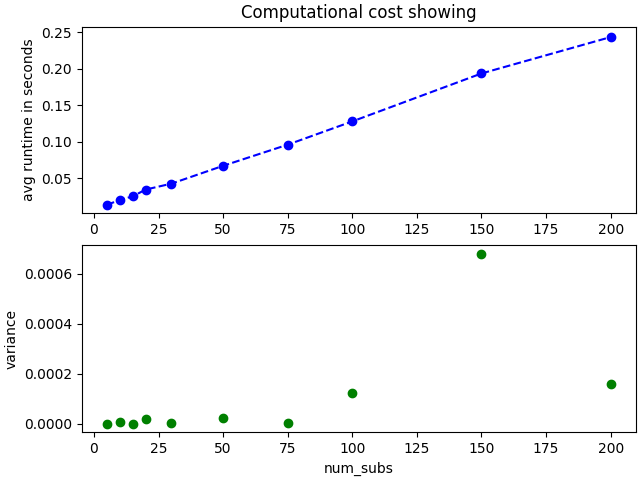
\includegraphics[width=0.49\linewidth]{../performance_analysis/runtime_showing.png}
    \caption{avg dataflow and runtime when requesting for the POI service}
    \label{fig:showing}
\end{figure}

\begin{figure}[h!]
    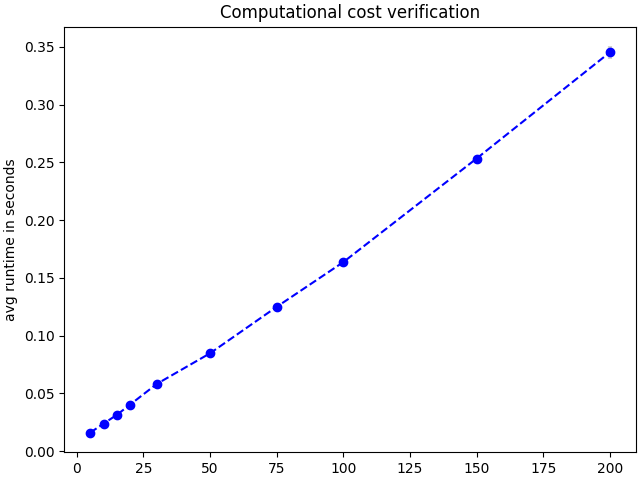
\includegraphics[width=0.49\linewidth]{../performance_analysis/runtime_verification}
    \caption{avg runtime for the credential verifications}
    \label{fig:verify}
\end{figure}


\section{(De)Anonymization of User Trajectories}

\subsection{Privacy Evaluation}
In this section, we performed a privacy evaluation on the network level of SecretStroll application. We showed how valuable metadata and side information, like IP addresses or location coordinates at query time, can be valuable for an adversary who aims to break users' anonymity. We also provided a countermeasure to try defending against the following attacks.


\subsubsection{Identity Inference Attack}


\paragraph{Threat Model}
For this attack, we considered a \textbf{passive} adversary (i.e \textit{Honest but Curious}). We modelled the adversary as \textbf{global} (i.e she has a full view of the network used by the system, meaning that she can eavesdrop queries made from whichever cell in SecretStroll grid. The adversarial view is represented by \textttt{queries.csv} dataset). More specifically, the adversary in this setting is SecretStroll \textbf{service provider}.\newline
We assumed the following background knowledge for the adversary: the adversary knows a mapping between users' IP addresses and their name and surname.\newline
We assumed the adversary computational power to be bounded by Polynomial time.


\paragraph{Adversarial Goal}
The goal of the adversary is to infer users' \textbf{top-3 locations}, namely their home location, their workplace location, and any particular place where they spend their leisure time. By knowing such sensible information and combining with her background knowledge, the adversary can uniquely identify users.


\paragraph{Implementation Details}
\begin{itemize}
    \item \textbf{Feature Extraction}: the first step for performing the attack was a simple process of feature extraction. We added 3 new columns to the \textit{queries.csv} dataset from the \textit{timestamp} column: \textit{hour} column, representing the hour of the day of the query,
    \textit{day} column, representing the day of the query and \textit{daytime} column, representing the
    daytime of the query (for example, a query launched at 10 a.m was labelled as "Morning", whereas a query launched at 10 p.m was labelled as "Night").
    \item \textbf{Trajectory Analysis}: the second step (optional) was to analyze the "quality" of the provided data: generally, when performing inference on users home or workplace location, the common assumption is that users follow a pattern, meaning that queries collected during the measurements will be launched from a small set of locations per user. Before mounting the attack, we decided to test this assumption. We collected, for each IP address, their daily trajectory (as a time-ordered sequence of latitude and longitude coordinates). We then computed the distance matrix between each pair of daily trajectories using \textit{Frechet Distance}.
    The results showed that, for each users, trajectories were very similar. Furthermore we could assess that \textit{Frechet Distance} represented a meaningful metric, since for each user we could witness a larger distance between trajectories collected during week days and trajectories collected during weekends (as expected by the different pattern of average people during work days compared to the one during days off).


    \begin{figure}[h!]
    \includegraphics[width=0.49\linewidth]{../privacy_evaluation/daily_trajectories/}
    \caption{Distance matrix for user TO BE CHOSEN trajectories}
    \label{fig:matrix}
    \end{figure}


    \item \textbf{Location clustering}: After validating the data, we proceeded to mount the attack. The attack consisted in a simple analysis on the dataset. We first grouped the daytimes we defined in three groups: the first group, \textit{daytime home}, is comprehensive of daytimes "Early" and "Night". Similarly, \textit{daytime work}, comprehends daytimes "Morning" and "Afternoon", while \textit{daytime leisure} the "Evening". Then, for each user, for each daytime group, we filtered queries accordingly and extracted latitudes and longitudes of locations. Then, we fed the coordinates, converted to radians, to the \textbf{DBSCAN} algorithm. After the clusters were formed, we extracted the most numerous one and computed the centroid. Hence, the home location for one user, for example, resulted to be the centroid of the cluster computed with queries filtered by daytime "home". Results are provided in the \textttt{top\_locations.csv} file. It is worth noticing that. for a few users, there were not enough queries during the "Evening" to infer something about their "leisure time" top location.
\end{itemize}

\subsubsection{De-anonimization of trajectories trough Co-Location}


\paragraph{Threat Model}
For this attack, similarly to the previous one, we considered the adversary to be the \textbf{service provider}. The adversary is thus again a \textbf{passive}, \textbf{global} one, wuth computational power bounded by polynomial time.\newline
As far as her background knowledge is concerned, we assumed that the adversary knows the names and surnames of a subset of users. Furthermore, we assumed that the adversary has access to a channel of side information about users, more concretely to users' public profiles on social networks.


\paragraph{Adversarial Goal}
The goal of the adversary is to infer the identiy of users for which she does not know a name-IP address mapping. In order to do so, the adversary looks for similarity, on daily basis, on users trajectories, in order to exploit the co-location information provided by her source of side information like the social network profiles. Suppose that IP address "IP A" belongs to a user for whom the adversary knows the identity, Alice. After running the attack, the adversary knows
that. on day 6, Alice trajectory was very similar to the one of user with ip address "IP B". The adversary exploits her background knowledge and discovers, visiting Alice public profile, that, on day 6, Alice spent the day with her friend Bob. The adversary can thus infer with good probability that user having "IP B" is Bob.

\paragraph{Implementation Details}
We adopted an approach very similar to step 2 of the previous attack. For each day, we collected each user trajectory. For users whose trajectories were made up of fewer points than the longest trajectory of the day, the last known position was used as padding. We then computed the distance matrix between trajectories, using again \textit{Frechet Distance}. Finally, we used \textbf{DSBSCAN} algorithm in order to find clusters within the trajectories. We reported, for each day where a cluster of size greater than one was found, the users whose trajectories belonged to the same cluster, and the day. The results are provided in the \textttt{users\_trajectories\_similarities.csv} file.


\subsection{Defences}
Propose a defence that users of the service could deploy to protect their privacy.  You
should state your assumptions, adversary models, and provide an experimental evaluation of your
defences using the datasets and the grid specification. You should also discuss the
privacy-utility trade-offs of your defence.

\section{Cell Fingerprinting via Network Traffic Analysis}

\subsection{Implementation details}
Provide a description of your implementation here. You should provide details on your data collection methods, feature extraction, and classifier training.

\subsection{Evaluation}
Provide an evaluation of your classifier here -- the metrics after 10-fold cross validation.

\subsection{Discussion and Countermeasures}
Comment on your findings here. How well did your classifier perform? What factors could influence its performance? Are there countermeasures against this kind of attack?

\bibliographystyle{IEEEtran}
\bibliography{bib}
\end{document}
